% Options for packages loaded elsewhere
% Options for packages loaded elsewhere
\PassOptionsToPackage{unicode}{hyperref}
\PassOptionsToPackage{hyphens}{url}
\PassOptionsToPackage{dvipsnames,svgnames,x11names}{xcolor}
%
\documentclass[
  letterpaper,
  DIV=11,
  numbers=noendperiod]{scrartcl}
\usepackage{xcolor}
\usepackage{amsmath,amssymb}
\setcounter{secnumdepth}{-\maxdimen} % remove section numbering
\usepackage{iftex}
\ifPDFTeX
  \usepackage[T1]{fontenc}
  \usepackage[utf8]{inputenc}
  \usepackage{textcomp} % provide euro and other symbols
\else % if luatex or xetex
  \usepackage{unicode-math} % this also loads fontspec
  \defaultfontfeatures{Scale=MatchLowercase}
  \defaultfontfeatures[\rmfamily]{Ligatures=TeX,Scale=1}
\fi
\usepackage{lmodern}
\ifPDFTeX\else
  % xetex/luatex font selection
\fi
% Use upquote if available, for straight quotes in verbatim environments
\IfFileExists{upquote.sty}{\usepackage{upquote}}{}
\IfFileExists{microtype.sty}{% use microtype if available
  \usepackage[]{microtype}
  \UseMicrotypeSet[protrusion]{basicmath} % disable protrusion for tt fonts
}{}
\makeatletter
\@ifundefined{KOMAClassName}{% if non-KOMA class
  \IfFileExists{parskip.sty}{%
    \usepackage{parskip}
  }{% else
    \setlength{\parindent}{0pt}
    \setlength{\parskip}{6pt plus 2pt minus 1pt}}
}{% if KOMA class
  \KOMAoptions{parskip=half}}
\makeatother
% Make \paragraph and \subparagraph free-standing
\makeatletter
\ifx\paragraph\undefined\else
  \let\oldparagraph\paragraph
  \renewcommand{\paragraph}{
    \@ifstar
      \xxxParagraphStar
      \xxxParagraphNoStar
  }
  \newcommand{\xxxParagraphStar}[1]{\oldparagraph*{#1}\mbox{}}
  \newcommand{\xxxParagraphNoStar}[1]{\oldparagraph{#1}\mbox{}}
\fi
\ifx\subparagraph\undefined\else
  \let\oldsubparagraph\subparagraph
  \renewcommand{\subparagraph}{
    \@ifstar
      \xxxSubParagraphStar
      \xxxSubParagraphNoStar
  }
  \newcommand{\xxxSubParagraphStar}[1]{\oldsubparagraph*{#1}\mbox{}}
  \newcommand{\xxxSubParagraphNoStar}[1]{\oldsubparagraph{#1}\mbox{}}
\fi
\makeatother


\usepackage{longtable,booktabs,array}
\usepackage{calc} % for calculating minipage widths
% Correct order of tables after \paragraph or \subparagraph
\usepackage{etoolbox}
\makeatletter
\patchcmd\longtable{\par}{\if@noskipsec\mbox{}\fi\par}{}{}
\makeatother
% Allow footnotes in longtable head/foot
\IfFileExists{footnotehyper.sty}{\usepackage{footnotehyper}}{\usepackage{footnote}}
\makesavenoteenv{longtable}
\usepackage{graphicx}
\makeatletter
\newsavebox\pandoc@box
\newcommand*\pandocbounded[1]{% scales image to fit in text height/width
  \sbox\pandoc@box{#1}%
  \Gscale@div\@tempa{\textheight}{\dimexpr\ht\pandoc@box+\dp\pandoc@box\relax}%
  \Gscale@div\@tempb{\linewidth}{\wd\pandoc@box}%
  \ifdim\@tempb\p@<\@tempa\p@\let\@tempa\@tempb\fi% select the smaller of both
  \ifdim\@tempa\p@<\p@\scalebox{\@tempa}{\usebox\pandoc@box}%
  \else\usebox{\pandoc@box}%
  \fi%
}
% Set default figure placement to htbp
\def\fps@figure{htbp}
\makeatother

\ifLuaTeX
  \usepackage{luacolor}
  \usepackage[soul]{lua-ul}
\else
  \usepackage{soul}
\fi




\setlength{\emergencystretch}{3em} % prevent overfull lines

\providecommand{\tightlist}{%
  \setlength{\itemsep}{0pt}\setlength{\parskip}{0pt}}



 


\KOMAoption{captions}{tableheading}
\makeatletter
\@ifpackageloaded{caption}{}{\usepackage{caption}}
\AtBeginDocument{%
\ifdefined\contentsname
  \renewcommand*\contentsname{Table of contents}
\else
  \newcommand\contentsname{Table of contents}
\fi
\ifdefined\listfigurename
  \renewcommand*\listfigurename{List of Figures}
\else
  \newcommand\listfigurename{List of Figures}
\fi
\ifdefined\listtablename
  \renewcommand*\listtablename{List of Tables}
\else
  \newcommand\listtablename{List of Tables}
\fi
\ifdefined\figurename
  \renewcommand*\figurename{Figure}
\else
  \newcommand\figurename{Figure}
\fi
\ifdefined\tablename
  \renewcommand*\tablename{Table}
\else
  \newcommand\tablename{Table}
\fi
}
\@ifpackageloaded{float}{}{\usepackage{float}}
\floatstyle{ruled}
\@ifundefined{c@chapter}{\newfloat{codelisting}{h}{lop}}{\newfloat{codelisting}{h}{lop}[chapter]}
\floatname{codelisting}{Listing}
\newcommand*\listoflistings{\listof{codelisting}{List of Listings}}
\makeatother
\makeatletter
\makeatother
\makeatletter
\@ifpackageloaded{caption}{}{\usepackage{caption}}
\@ifpackageloaded{subcaption}{}{\usepackage{subcaption}}
\makeatother
\usepackage{bookmark}
\IfFileExists{xurl.sty}{\usepackage{xurl}}{} % add URL line breaks if available
\urlstyle{same}
\hypersetup{
  pdftitle={-Better software for Better research- Introduction to the FAIR2 for Research Software training Programme},
  pdfauthor={ Romain Thomas Head of Research Software Engineering,  The University of Sheffield rse.shef.ac.uk},
  colorlinks=true,
  linkcolor={blue},
  filecolor={Maroon},
  citecolor={Blue},
  urlcolor={Blue},
  pdfcreator={LaTeX via pandoc}}


\title{-Better software for Better research-Introduction to the FAIR2
for Research Software training Programme}
\author{\textbf{Romain Thomas}\href{https://rse.shef.ac.uk/}{Head of
Research Software Engineering}, The University of
Sheffield\href{https://rse.shef.ac.uk}{rse.shef.ac.uk}}
\date{}
\begin{document}
\maketitle


\subsection{Useful Information:}\label{useful-information}

\begin{itemize}
\item
  This talk is recorded.
\item
  You can follow the slides {➡️}{➡️}
\item
  Slides are available freely on github.
\item
  You can interupt me at any moment if you have a question.
\item
  Every \href{}{blue} text is a hyperlink.
\end{itemize}

\begin{center}
\pandocbounded{\includegraphics[keepaspectratio]{assets/images/FAIR_slides.png}}
\end{center}

\subsection{Who am I?}\label{who-am-i}

\begin{itemize}
\item
  Name : Romain Thomas
\item
  Role : Head of Research Software Engineering
\item
  Previously : Staff Astronomer and Software Project manager at the Very
  Large Telescope (Chile)
\item
  Released/Published a few modules/software:

  \begin{itemize}
  \tightlist
  \item
    \href{https://github.com/Romain-Thomas-Shef/STON}{STON} (submitted,
    JOSS)
  \item
    \href{https://joss.theoj.org/papers/10.21105/joss.01249}{dfitspy}
  \item
    \href{https://www.spiedigitallibrary.org/conference-proceedings-of-spie/11449/2560271/The-SCUBA-project---First-layer-of-quality-control/10.1117/12.2560271.full}{SCUBA}
  \item
    \href{https://www.sciencedirect.com/science/article/pii/S2213133720300810?via\%3Dihub}{SPARTAN}
  \end{itemize}
\end{itemize}

\includegraphics[width=8.33333in,height=2.60417in]{assets/images/p3.jpg}

\subsection{Who are we? The teams behind the
programme}\label{who-are-we-the-teams-behind-the-programme}

\textbf{Research Software Engineering}

\begin{center}
\pandocbounded{
\includegraphics[keepaspectratio]{index_files/mediabag/assets/images/RSE_logo_blackborder.pdf}}
\end{center}

The Research Software Engineering team is composed of 13 members and
{\textbf{collaborates with researchers across the University in building
research software}}. Areas of expertise within the group include:
general software development, code optimisation and performance,
reproducibility, GPU computing and Deep Learning, High Performance
Computing, training, etc\ldots{}

\subsection{Who are we? The teams behind the
programme}\label{who-are-we-the-teams-behind-the-programme-1}

\textbf{Data Analytics Service}

\includegraphics[width=3.125in,height=0.9375in]{assets/images/DAS_logo.png}

The Data Analytics Service (IT Services) supports research excellence at
the University of Sheffield by bridging technical and analytical gaps
through consultation, delivering training, and long-term collaboration
with research teams. {DAS supports researchers with reproducible data
analysis, data visualisation, data engineering, machine learning,
statistics, big data, research software, web design, and much more.}

\subsection{Who are we? The teams behind the
programme}\label{who-are-we-the-teams-behind-the-programme-2}

\textbf{Library's Scholarly Communications}

\includegraphics[width=3.125in,height=0.625in]{assets/images/Library_logo_violet_white.png}

The Library's Scholarly Communications Team provides specialist services
to support researchers at the University of Sheffield. They offer
guidance on making your research outputs open access, and give {support
on good practice in research data management, copyright and licensing as
well as open research more broadly.}

\subsection{This is our second year!}\label{this-is-our-second-year}

During our first delivery we have seen \textasciitilde250 registrations
to our training programme from all Faculties at the university.
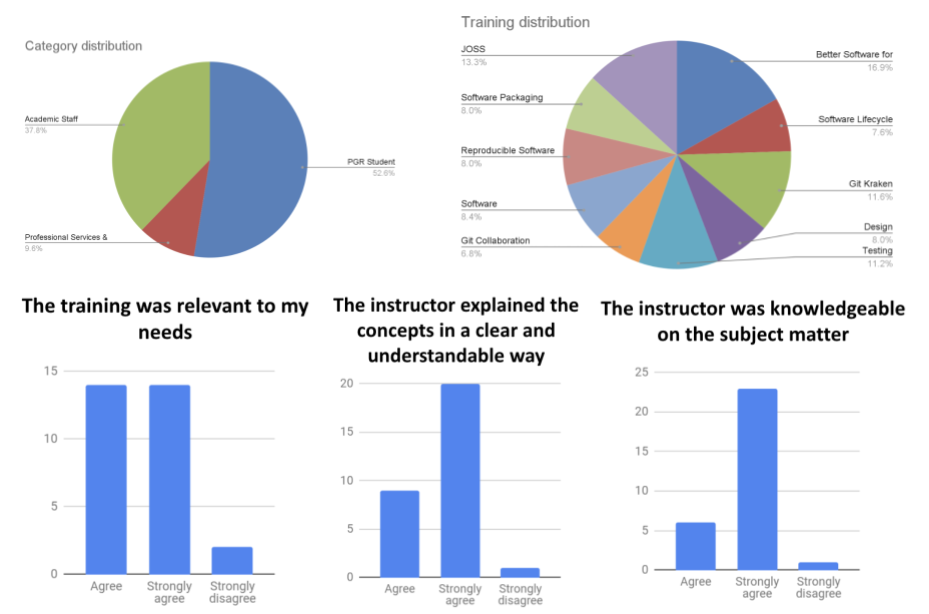
\includegraphics[width=9.375in,height=5.20833in]{assets/images/Recap24.png}

\subsection{Programme very well received
!!!}\label{programme-very-well-received}

\begin{itemize}
\tightlist
\item
  \emph{``Very clear explanations, which was great because my depth of
  knowledge of software development is varied. It's helpful to have the
  foundations explained clearly.''}
\item
  \emph{``I really liked having presentations from multiple different
  people from across the university within one session.''}
\item
  \emph{``I appreciated that time was set aside to put the learning into
  practice''}
\item
  \emph{``It reinforced many of the software development rules and ideas
  that will help with future development''}
\end{itemize}

\subsection{We are starting teaching it
now!}\label{we-are-starting-teaching-it-now}

\begin{itemize}
\tightlist
\item
  This second year also sees us \textbf{teaching} a (shortened) version
  of our programme to the made4manufacturing CDT.
\item
  Part of the Data Science and RSE module.
\end{itemize}

\section{Why FAIR?}\label{why-fair}

\section{\texorpdfstring{Why \st{FAIR}?}{Why FAIR?}}\label{why-fair-1}

\section{Why OPEN?}\label{why-open}

\subsection{Research is a continuous
process}\label{research-is-a-continuous-process}

{``The succession of researchers is comparable to a single person who
learns indefinitely.} \emph{Pascal, Pensee, French Mathematician,
Physicist, inventor, philosopher and theologian {[}1623-1662{]}}
\includegraphics[width=3.125in,height=3.64583in]{assets/images/pascal.webp}

\begin{itemize}
\tightlist
\item
  That's very old\ldots.
\item
  But still very valid\ldots{}
\item
  And becomes much more difficult with thecomplexity of modern research
\end{itemize}

\subsection{Research creates knowledge\ldots that is passed
down}\label{research-creates-knowledgethat-is-passed-down}

{``Knowledge is humankind's most precious treasure. Everything that we
accomplished has been done due to the capacity to create a transmissible
heritage, which spares each new generation the task of starting from
scratch.''} \emph{B. Sirbey, le grand homme qui apprend.}

\begin{quote}
If we are doing the research we are doing today, it is thanks to the
work of previous generations that created the knowledge that we are
using now.
\end{quote}

\subsection{And that can be
trusted\ldots{}}\label{and-that-can-be-trusted}

\begin{itemize}
\tightlist
\item
  Research relies on the ability to trust what has been done before.
\item
  This means that a result has been tested, verified and could be
  {reproduced} {➡️}{➡️}
\item
  Tools and methods used for a particular result are known and
  shared\ldots{}
\end{itemize}

\pandocbounded{\includegraphics[keepaspectratio]{assets/images/reproducible_turing.png}}
\href{https://the-turing-way.netlify.app/reproducible-research/rdm/rdm-fair.html}{The
Turing Way} project illustration by Scriberia. Used under a CC-BY 4.0
licence. DOI:
\href{https://dx.doi.org/10.5281/zenodo.3332807}{10.5281/zenodo.3332807}

\subsection{What if a generation of researchers stop doing
this?}\label{what-if-a-generation-of-researchers-stop-doing-this}

\begin{itemize}
\tightlist
\item
  Tools and methods used for a particular results are {NOT} known and
  shared\ldots{}
\item
  This means that a result can {NOT} be tested and verified and can
  {NOT} be reproduced.
\item
  {➡️} It is harder to trust research
\end{itemize}

\pandocbounded{\includegraphics[keepaspectratio]{assets/images/reproducible_turing.png}}
\href{https://the-turing-way.netlify.app/reproducible-research/rdm/rdm-fair.html}{The
Turing Way} project illustration by Scriberia. Used under a CC-BY 4.0
licence. DOI:
\href{https://dx.doi.org/10.5281/zenodo.3332807}{10.5281/zenodo.3332807}

\subsection{Are we far from reaching this
situation?}\label{are-we-far-from-reaching-this-situation}

\pandocbounded{\includegraphics[keepaspectratio]{assets/images/NatureSurvey.png}}

\href{https://www.nature.com/articles/533452a}{Source: Baker M., Nature,
2016}

\begin{itemize}
\tightlist
\item
  90\% said there is a crisis!
\item
  More than 70\% of researchers have tried and failed to reproduce
  another scientist's experiments\ldots{}
\item
  {And more than half have failed to reproduce their own experiments.}
\end{itemize}

\includegraphics[width=6.25in,height=3.125in]{assets/images/Joey.png}

\section{So how do we get better?}\label{so-how-do-we-get-better}

\subsection{Let's improve!}\label{lets-improve}

\begin{center}
\pandocbounded{\includegraphics[keepaspectratio]{assets/images/continuum.png}}
\end{center}

\href{https://www.aalto.fi/en/open-science-and-research/getting-started-with-reproducibility-in-research}{Source:
www.aalto.fi}

\section{And why not start with your
software?}\label{and-why-not-start-with-your-software}

\subsection{Let's start by a definition: What is a
software?}\label{lets-start-by-a-definition-what-is-a-software}

``Source code files, algorithms, scripts, computational workflows and
executables that were created during the research process or for a
research purpose.''

\href{https://dx.doi.org/10.1038/s41597-022-01710-x}{Barker et
al.~Scientific Data 9:622 (2022) ``Introducing the FAIR Principles for
research software''}

\section{What is FAIR?}\label{what-is-fair}

\subsection{The FAIR principles}\label{the-fair-principles}

\begin{center}
\pandocbounded{\includegraphics[keepaspectratio]{assets/images/Fairprinciples.jpg}}
\end{center}
\href{https://the-turing-way.netlify.app/reproducible-research/rdm/rdm-fair.html}{The
Turing Way} project illustration by Scriberia. Used under a CC-BY 4.0
licence. DOI:
\href{https://dx.doi.org/10.5281/zenodo.3332807}{10.5281/zenodo.3332807}

A guideline for those wishing to enhance the reusability of their data
holdings \href{https://www.nature.com/articles/sdata201618}{--Wilkinson
et al.~(2016)--}

\subsection{The FAIR principles}\label{the-fair-principles-1}

``Many of the FAIR Guiding Principles can be directly applied to
research software by treating software and data as similar digital
research objects. However, {specific characteristics of software ---
such as its executability, composite nature, and continuous evolution
and versioning} --- make it necessary to revise and extend the
principles.''

\href{https://doi.org/10.15497/RDA00068}{Chue Hong, Neil P. et al, FAIR
Principles for Research Software (FAIR4RS Principles)}

\subsection{The FAIR principles: what do they
say?}\label{the-fair-principles-what-do-they-say}

\begin{itemize}
\item
  {Findable}: Software, and its associated metadata, is easy for both
  humans and machines to find
\item
  {Accessible}: Software, and its metadata, is retrievable via
  standardised protocols
\end{itemize}

\href{https://dx.doi.org/10.1038/s41597-022-01710-x}{Barker \emph{et
al.} \emph{Scientific Data} 9:622 (2022) ``Introducing the FAIR
Principles for research software'' DOI: 10.1038/s41597-022-01710-x}

FINDABLE: Research software should have a globally unique and persistent
identifier (e.g., DOI or a persistent URL) so that it can be easily
found and cited. Sufficient metadata should be provided to help users
discover the software. This includes descriptions of the software's
function, version information, authorship, and where to access it. The
software and its metadata should be indexed in searchable repositories
so it can be discovered via common search engines and research
infrastructure platforms (e.g., Zenodo, GitHub, or institutional
repositories).

ACCESSIBLE: The software should be easily retrievable using the unique
identifier. Typically, this involves storing the software in a trusted
repository that ensures long-term access. Clear information about the
conditions under which the software can be accessed should be available,
including open access options, if applicable. This ensures users
understand whether they can freely use or adapt the software.

\subsection{The FAIR principles: what do they
say?}\label{the-fair-principles-what-do-they-say-1}

\begin{itemize}
\item
  {Interoperable}: Software interoperates with other software by
  exchanging data and/or metadata, and/or through interaction via
  application programming interfaces (APIs), described through
  standards.
\item
  {Reusable}: Software is both usable (can be executed) and reusable
  (can be understood, modified, built upon, or incorporated into other
  software)
\end{itemize}

\href{https://dx.doi.org/10.1038/s41597-022-01710-x}{Barker \emph{et
al.} \emph{Scientific Data} 9:622 (2022) ``Introducing the FAIR
Principles for research software'' DOI: 10.1038/s41597-022-01710-x}

INTEROPERABLE: The software should use standardized data formats and
interfaces where possible, allowing it to work with other software,
tools, or systems. Clear documentation should be provided so users know
how to integrate the software with other tools or systems. Where
possible, the software should implement and support established
protocols, formats, and APIs that are widely adopted in the research
community.

REUSABLE: The software should be well-documented, including clear
instructions on how to install, run, and modify it. The metadata should
describe how and where the software can be reused, including
dependencies, versioning, and requirements. An appropriate open or
permissive license should be provided to ensure that others can legally
reuse, modify, and redistribute the software. Adhering to coding
standards, including the use of tests and continuous integration (CI),
enhances the reliability and reusability of the software.

\subsection{University's position about
FAIR}\label{universitys-position-about-fair}

``We aspire to open research culture that values a diverse range of
contributions and adheres to the FAIR principles to enable the results
of our research to be of maximum benefit to society (findable,
accessible, interoperable and reusable), whilst also respecting
circumstances that limit data sharing (for example, due to issues of
privacy, non-consent, contractual agreements, legislation or
practicality).'\,'\\
\href{https://www.sheffield.ac.uk/openresearch/university-statement-open-research}{University
of Sheffield, Statement on Open Research} ``All researchers, including
postgraduate research students, have a personal responsibility to manage
effectively the data they create\ldots.. All researchers are expected to
document research data and software in line with the FAIR
principles\ldots..'\,'\\
\href{https://www.sheffield.ac.uk/media/18953/download}{University of
Sheffield, Policy on good research and innovation practices}

\subsection{Barriers to FAIR24RS}\label{barriers-to-fair24rs}

\begin{itemize}
\tightlist
\item
  fear of prejudice

  \begin{itemize}
  \tightlist
  \item
    important to create a positive culture
  \end{itemize}
\item
  fear of `theft'

  \begin{itemize}
  \tightlist
  \item
    licensing and citation
  \end{itemize}
\item
  technical and time barriers

  \begin{itemize}
  \tightlist
  \item
    support is available!
  \item
    only need to learn once
  \end{itemize}
\item
  non-commercialisable?

  \begin{itemize}
  \tightlist
  \item
    open source and commercialisation are compatible
  \item
    greater impact through open source
  \end{itemize}
\end{itemize}

\pandocbounded{\includegraphics[keepaspectratio]{assets/images/keynote1h.JPG}}
\href{https://doi.org/10.6084/m9.figshare.5558653.v1}{Better Science
through Better Data 2017) scribe images.}

\subsection{Benefits of FAIR24RS}\label{benefits-of-fair24rs}

\pandocbounded{\includegraphics[keepaspectratio]{assets/images/keynote1b.JPG}}
\href{https://doi.org/10.6084/m9.figshare.5558653.v1}{Better Science
through Better Data 2017) scribe images.}

\begin{itemize}
\tightlist
\item
  Accelerate research
\item
  Increase transparency of research
\item
  Increase visibility, citation, reputation and impact
\item
  Reduce duplication of effort
\end{itemize}

\subsection{How to be FAIR?}\label{how-to-be-fair}

\begin{center}
\includegraphics[width=8.33333in,height=5.20833in]{assets/images/chan_invert.png}
\end{center}

\subsection{\texorpdfstring{FA{IR}4RS: Think about how you are
coding\ldots{}}{FAIR4RS: Think about how you are coding\ldots{}}}\label{fair4rs-think-about-how-you-are-coding}

\begin{itemize}
\tightlist
\item
  Where possible, make your code modular.
\item
  Comment your code to make it as clear as possible.
\item
  Create and provide tests that others can use.
\item
  Follow code standards
\end{itemize}

\includegraphics[width=5.20833in,height=3.64583in]{assets/images/C++style.png}
\includegraphics[width=4.16667in,height=1.5625in]{assets/images/RStyle.png}
\includegraphics[width=4.16667in,height=1.5625in]{assets/images/PEP8.png}

\subsection{\texorpdfstring{FA{IR}4RS: Be open even inside the
code!}{FAIR4RS: Be open even inside the code!}}\label{fair4rs-be-open-even-inside-the-code}

\begin{itemize}
\tightlist
\item
  Where possible and applicable, outputs (even between pieces of code)
  should use open and accessible data formats, which will help if other
  researchers only wish to use part of your code.
\item
  {But do NOT reinvent the wheel!} In some research fields data format
  are standardized {➡️} if you want people to use your code, use
  {[}your{]} community standards!
\end{itemize}

\includegraphics[width=5.20833in,height=3.64583in]{assets/images/wheel.png}

\subsection{\texorpdfstring{{FAIR}4RS: Version your
code!}{FAIR4RS: Version your code!}}\label{fair4rs-version-your-code}

\begin{itemize}
\tightlist
\item
  Using version control software platform such as Github/GitLab allows
  you to keep track of the changes you make to your code
\item
  You can release version of your software/code/scripts directly from
  Github. While it should not be used a long term storage place, It
  gives a place where your code can be downloaded and where people can
  contribute.
\end{itemize}

\includegraphics[width=5in,height=3.125in]{assets/images/repo.png}
\url{https://www.sheffield.ac.uk/library/research-data-management/repositories}

\subsection{\texorpdfstring{FA{IR}4RS: Document your
code!}{FAIR4RS: Document your code!}}\label{fair4rs-document-your-code}

A little poem from
\href{https://www.writethedocs.org/guide/writing/beginners-guide-to-docs/\%5D}{A
beginner's guide to writing documentation}:

\begin{itemize}
\tightlist
\item
  If people don't know why your project exists, they won't use it.
\item
  If people can't figure out how to install your code, they won't use
  it.
\item
  If people can't figure out how to use your code, they won't use it.
\end{itemize}

\subsection{\texorpdfstring{FA{IR}4RS: Document your
code!}{FAIR4RS: Document your code!}}\label{fair4rs-document-your-code-1}

A little poem from
\href{https://www.writethedocs.org/guide/writing/beginners-guide-to-docs/\%5D}{A
beginner's guide to writing documentation}:

\begin{itemize}
\tightlist
\item
  If people don't know why your project exists, they won't use it.
\item
  If people can't figure out how to install your code, they won't use
  it.
\item
  If people can't figure out how to use your code, they won't use it.
\end{itemize}

In practice, Github can host documentation as website (and it is very
easy to do!) {➡️}{➡️}

\includegraphics[width=5.20833in,height=3.64583in]{assets/images/RSEwebsite.png}
\includegraphics[width=4.16667in,height=2.60417in]{assets/images/rtd.jpg}

\subsection{\texorpdfstring{FA{IR}4RS: Licence your
code!}{FAIR4RS: Licence your code!}}\label{fair4rs-licence-your-code}

You need to tell people how they can re-use your code.

\begin{itemize}
\tightlist
\item
  GPLv3 \href{https://www.gnu.org/licenses/gpl-3.0.en.html}{The GNU
  General Public License}: a free, copyleft license for software and
  other kinds of works. It is intended to guarantee your freedom to
  share and change all versions of a software to make sure it remains
  free software for all its users
\item
  \href{https://opensource.org/license/mit/}{MIT licence}: is a
  permissive free software license. Without limitation the rights to
  use, copy, modify, merge, publish, distribute, sublicense, and/or sell
  copies of the Software,
\end{itemize}

\includegraphics[width=5.20833in,height=2.91667in]{assets/images/licence.png}

{The licence must be made clear in the code repository and in the
documentation.}

\subsection{\texorpdfstring{FA{IR}4RS: Get credit for your
work}{FAIR4RS: Get credit for your work}}\label{fair4rs-get-credit-for-your-work}

If people are using your software you should get credit for it.

{➡️} state how you want to be credited. You can add it in the
documentation and/or create a
\href{https://citation-file-format.github.io/}{citation.cff} file that
you can add with your code
(\href{https://citation-file-format.github.io/cff-initializer-javascript/\#/}{tools}.
are available to generate them)

\includegraphics[width=5.20833in,height=2.91667in]{assets/images/citation_cff.png}
\includegraphics[width=5.20833in,height=2.08333in]{assets/images/acknow.png}

\subsection{\texorpdfstring{FA{IR}4RS: Share
it!}{FAIR4RS: Share it!}}\label{fair4rs-share-it}

\begin{itemize}
\tightlist
\item
  Create a description of your code with metadata {[}data about your
  software{]}.
\item
  Codemeta is a set of keywords used to describe code and how to
  structure them in a machine readable way
\end{itemize}

Examples:

\begin{itemize}
\tightlist
\item
  The citation.cff file contains metadata
\item
  Description keywords
\item
  Url to repository, to documentation
\item
  List of contributors and affiliations
\item
  etc\ldots{}
\end{itemize}

\includegraphics[width=4.16667in,height=3.125in]{assets/images/metadata.png}

\subsection{\texorpdfstring{FA{IR}4RS: Share
it!}{FAIR4RS: Share it!}}\label{fair4rs-share-it-1}

In order to ensure that others can access and download your code, and
that this access remains permanent over time, you should deposit your
code in a repository. Two types:

\begin{itemize}
\tightlist
\item
  General purpose
\item
  Domain Specific
\end{itemize}

{ Choose what makes more sense for you project! }

\includegraphics[width=5.20833in,height=3.125in]{assets/images/zenodo.png}

\subsection{\texorpdfstring{FA{IR}4RS: Share
it!}{FAIR4RS: Share it!}}\label{fair4rs-share-it-2}

In order to ensure that others can access and download your code, and
that this access remains permanent over time, you should deposit your
code in a repository. Two types:

\begin{itemize}
\tightlist
\item
  General purpose
\item
  Domain Specific
\end{itemize}

{Choose what makes more sense for you project!}

\includegraphics[width=4.16667in,height=2.08333in]{assets/images/re3.png}

{Numerous repositories give your content a DOI {[}Digital Object
Identifier{]}} It means it can be cited in publication and other
communications in order to open up your research to others and invite
collaboration, as well as ensuring a constant link to your code.

\subsection{\texorpdfstring{{FA}IR4RS: Publish
it!}{FAIR4RS: Publish it!}}\label{fair4rs-publish-it}

\begin{itemize}
\tightlist
\item
  Generalist software journals

  \begin{itemize}
  \tightlist
  \item
    \href{https://joss.theoj.org/}{JOSS}: Journal of Open Source
    Software: Academic journal with a formal peer review process that is
    designed to improve the quality of the software submitted.
  \item
    \href{https://openresearchsoftware.metajnl.com/}{JORS}: Journal of
    Open Research Software: Features peer reviewed Software Metapapers
    describing research software with high reuse potential.
  \item
    \href{https://www.sciencedirect.com/journal/software-impacts}{Software
    Impacts}: multidisciplinary, open access, peer-reviewed journal
    which publishes short, articles that describe software which
    addresses a research challenge.
  \end{itemize}
\end{itemize}

\begin{itemize}
\tightlist
\item
  Some are domain specific:

  \begin{itemize}
  \tightlist
  \item
    Astronomy and computing
  \item
    Journal of Artificial Societies and Social Simulation
  \item
    Journal of Statistical Software
  \item
    Science of Computer Programming
  \item
    Computer Methods and Programs in Biomedicine
  \end{itemize}
\end{itemize}

You can find a list of potential journals
\href{https://www.software.ac.uk/top-tip/which-journals-should-i-publish-my-software}{here}

\section{The FAIR24RS training programme at the
University}\label{the-fair24rs-training-programme-at-the-university}

\subsection{Lack of skills for developing
software}\label{lack-of-skills-for-developing-software}

Do you feel that you have received sufficient training to develop
reliable software?

Bob Turner \& Paul Richmond, UoS, RSE team,
\href{rse.shef.ac.uk/sssurvey}{github.com/RSE-Sheffield/sssurvey}.

\includegraphics[width=5.20833in,height=2.08333in]{assets/images/Survey.png}

\subsection{The FAIR24RS Programme:
Overview}\label{the-fair24rs-programme-overview}

\begin{center}
\pandocbounded{\includegraphics[keepaspectratio]{assets/images/Programme.png}}
\end{center}

\subsection{Version control: Git, GitHub and GitKraken - From Zero to
Hero}\label{version-control-git-github-and-gitkraken---from-zero-to-hero}

{Who}: \href{mailto:m.foster@sheffield.ac.uk}{Michael Foster} \& Dan
Brady

{When/Length}: 18/19 November (2 half days). Another session in February

{Format}: In person

Abstract:

If you've never heard of or used version control and Git before this is
the course for you. We start by introducing version control and
exploring how it can be beneficial to researchers, then we introduce
some useful tools and get started with some basic workflow using these
tools. We build on those foundations with collaborative exercises that
introduce key concepts such as forks, pull requests and branches and
give you the chance to {\emph{get some hands-on experience with using
version control in a research setting}}.

\subsection{{[}Advanced{]} Version control: Git with
it!}\label{advanced-version-control-git-with-it}

{Who}: \href{mailto:neil.shephard@sheffield.ac.uk}{Neil Shephard}

{When/Length}: February

{Format}: In person

Abstract:

This course aims to help you develop a {\emph{deeper understanding of
how Git works to facilitate collaboration}}. It builds on foundations
laid by the Git beginners course. The core idea around the course is
that by improving your understanding of working with branches and how to
make your commits tidier and neater it makes it easier to understand
pull requests and Git history which in turn makes it easier to
collaborate and work on code with others (including your future self!).

\subsection{Design your code (and write less of
it)}\label{design-your-code-and-write-less-of-it}

{Who}: \href{mailto:martin.dyer@sheffield.ac.uk}{Martin Dyer} \& Neil
Shephard

{When/Length}: 26/11 \& 03/12 (2 half days)

{Format}: In person

Abstract:

The way you write your code will have a massive impact on how easy it is
to maintain in the long run. {\emph{This course on Code Design
introduces essential principles and best practices for writing clean and
maintainable code}}. We will learn how we can write clean code, adhering
to naming conventions, commenting, and following PEP 8 guidelines. We
will then explore some fundamental principles such as DRY, KISS or YAGNI
that are important to keep in mind when writing new code and see how we
can spend less time touching the code by introducing configuration files
and command line interface.

\subsection{Software Lifecycle
Planning}\label{software-lifecycle-planning}

{Who}: \href{mailto:romain.thomas@sheffield.ac.uk}{R Thomas}, \href{}{R.
Campbell}, \href{}{K. O'Neill}

{When/Length}: 11/12, \textasciitilde2.5h (afternoon)

{Format}: Online

Abstract:

When you start writing software it is often very useful to think about
the development process and how you will make your software sustainable
in the long term. In this module we will introduce important aspects of
software development in research: {\emph{software management plan,
licences and dissemination}}. This module should allow you to ask
yourself the right questions when starting a research software project.

\subsection{Code Testing}\label{code-testing}

{Who}: \href{mailto:sylvia.whittle@sheffield.ac.uk}{Sylvia Whittle} \&
Michael Foster

{When/Length}: January (half day)

{Format}: In person

Abstract:

Does your code work? Are you sure? How do you ensure that it keeps
working when you change it? Manually verifying is slow and tedious. Why
not automate it? Software testing checks that your code works for you,
and when it breaks, it can show you exactly where it broke, without you
having to trawl through hundreds of lines of code manually.{\emph{This
course aims to provide you with the tools you need to start
automatically ensuring the reliability of your code.}}

\subsection{Documentation}\label{documentation}

{Who}: \href{mailto:joe.heffer@sheffield.ac.uk}{Joe Heffer}

{When/Length}: February (half day)

{Format}: In person

Abstract:

Well-documented software promotes reproducibility, maintainability, and
increased research impact through wider adoption and citation.
{\emph{This course teaches researchers how to document their software
effectively, making it accessible and understandable to others.}} It
covers topics such as writing readable code and usage instructions.

\subsection{Reproducible Environments}\label{reproducible-environments}

{Who}: \href{mailto:dan.brady@sheffield.ac.uk}{Dan Brady}

{When/Length}: March {[}half day{]}

{Format}: In person

Abstract:

Ensuring that others are able to take your code, run it, and are able to
produce the same (or equivalent) results is one of the key tenets of
FAIR and reproducible research software. {\emph{This course will provide
you with an overview of different ways to make your code reproducible}}
and then focus on virtual environments as a specific tool for
computational reproducibility.

\subsection{Packaging}\label{packaging}

{Who}: \href{}{Chris Wild} and \href{}{Farhad Allian}

{When/Length}: April {[}half day{]}

{Format}: In person

Abstract:

Packaging your software is one of the most important steps in a software
project to make it both findable and accessible. {\emph{This course will
provide you with an understanding of why and when packaging is useful}},
what different standards exist to package Python projects and take you
through each step of the packaging process.

\subsection{Software Papers}\label{software-papers}

{Who}: \href{mailto:romain.thomas@sheffield.ac.uk}{Romain Thomas}

{When/Length}: April, 45min

{Format}: Online

Abstract:

Did you know that you can actually publish a paper about your software?
This is an ideal way to get recognition (and citation) for the software
you have spent countless hours creating. {\emph{In this course we will
walk you through an example of submission in the
\href{https://joss.theoj.org/}{Journal of Open Source Software}.}} We
will make an example software submission to the journal, and thanks to
the collaboration of the Editor in Chief of JOSS (Arfon Smith), we will
look at how the review process is done.

\subsection{The FAIR24RS Programme:
Timeline}\label{the-fair24rs-programme-timeline}

\begin{center}
\pandocbounded{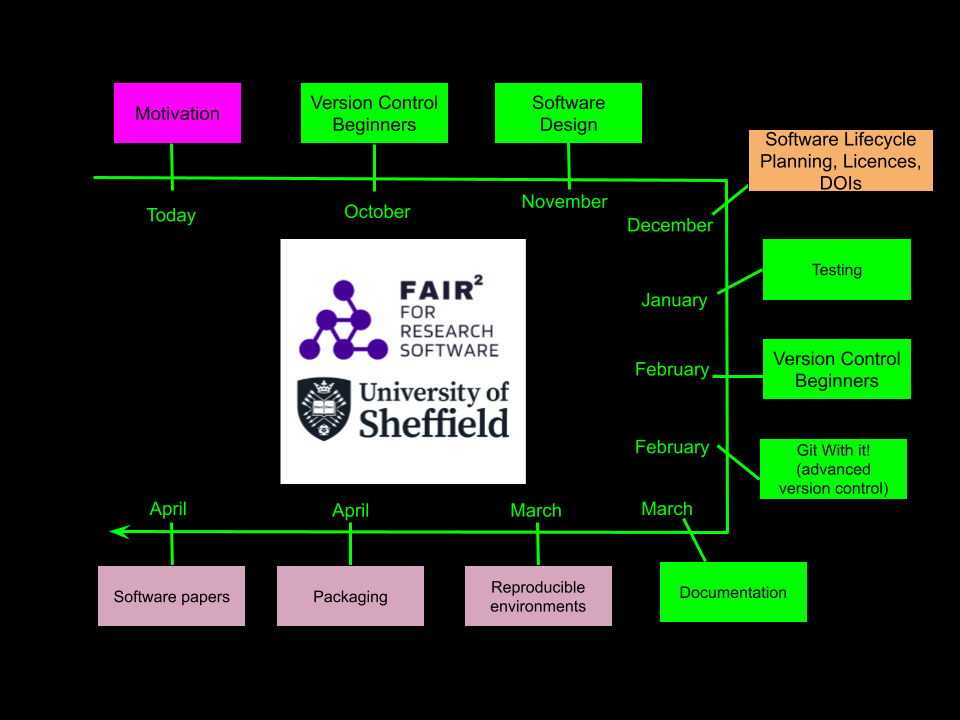
\includegraphics[keepaspectratio]{assets/images/FAIR_programme.png}}
\end{center}

\subsection{The FAIR24RS Programme: Material and
dependencies}\label{the-fair24rs-programme-material-and-dependencies}

\begin{itemize}
\item
  All materials are designed using the same structure
  (\href{https://carpentries.github.io/workbench/}{Software Carpentry
  workbench}) and are freely accessible on Github.
\item
  {\textbf{You can pick-and-choose the lecture}} you will follow based
  on the skills you already have. Each lecture comes with a set of
  prerequisities that are clearly identified.
\item
  A feedback form will be provided after each lecture.
\end{itemize}

\includegraphics[width=4.6875in,height=5.20833in]{assets/images/Example_course.png}

\subsection{the fair24rs programme: important
notes}\label{the-fair24rs-programme-important-notes}

\begin{itemize}
\tightlist
\item
  Training are all {Free of charge}.\\
\item
  BUT! they all need registration and {in-person sessions have limited
  places!}
\item
  They will all be available on mydevelopment platform. The first 3
  sessions are already open for registration:

  \begin{itemize}
  \tightlist
  \item
    \href{https://mydevelopment.csod.com/ui/lms-learning-details/app/event/d4d09f67-097b-4451-8ddb-86cb90636c06}{Git/Github
    zero to Hero} - Oct 28th \& Nov 4th
  \item
    \href{https://mydevelopment.csod.com/ui/lms-learning-details/app/event/d3c2cca5-d894-44b6-a79b-e93dea7a7c94}{Code
    Design} - Nov 26th \& Dec 3rd
  \item
    \href{https://mydevelopment.csod.com/ui/lms-learning-details/app/event/2d69f5c5-f9e7-46c2-999a-ffb3ed1db028}{Software
    Management plan} - Dec 12th
  \end{itemize}
\item
  January onward sessions will be available for booking around December.
\end{itemize}

\begin{itemize}
\tightlist
\item
  Direct links are also available on the RSE website:
\end{itemize}

\includegraphics[width=2.08333in,height=2.08333in]{assets/images/FAIR_rse_website.png}

\subsection{RSE website}\label{rse-website}

\begin{center}
\pandocbounded{\includegraphics[keepaspectratio]{assets/images/Screenshot_website.png}}
\end{center}

\textbf{Contacts:}

\begin{itemize}
\tightlist
\item
  Tamora James -RSE and FAIR24RS Programme Manager
  -\href{mailto:t.d.james@sheffield.ac.uk}{(t.d.james@sheffield.ac.uk)}
\item
  Romain Thomas -Head of
  RSE-\href{mailto:romain.thomas@sheffield.ac.uk}{(romain.thomas@sheffield.ac.uk)}
\end{itemize}

\subsection{Acknowledgements \&
References}\label{acknowledgements-references}

\begin{itemize}
\tightlist
\item
  Thank you to Tamora James for leading the development of this training
  programme
\item
  Thank you to Christopher Wild, Ric Campbell, Farhad Allian, Daniel
  Brady, Kate O'neill, Joe Heffer, Jenni Adams, Neil Shephard, Sylvia
  Wittle and Arfon Smith for dedicating time to prepare all the
  material!
\end{itemize}

\textbf{References} * D. Wilby
\href{https://www.davidwilby.dev/opensourcefair4rs/\#/title-slide}{Lunchbyte
talk on the FAIR principles} * T. James, FAIR for research software,
Talk OpenFest 2024 *
\href{https://book.the-turing-way.org/index.html}{The Turing Way} * B.
Sirvey
\href{https://medium.com/@borissirbey/le-grand-homme-qui-apprend-0bc4f4330d2d}{Le
grand homme qui apprend} * Chue Hong, Neil P. et al,
\href{https://doi.org/10.15497/RDA00068}{FAIR principles for Research
Software}

\subsection{Thank you!}\label{thank-you}

\begin{center}
\pandocbounded{\includegraphics[keepaspectratio]{assets/images/qr-code_feedback.png}}
\end{center}

Help us improve!

Scan to give your feedback!




\end{document}
